\documentclass{article}
%\documentclass[english,twoside]{article}
\usepackage[T1]{fontenc}
\usepackage{float}
\usepackage{graphicx}
\usepackage{minted}

% Set Document Font
% Only works using \XeLatex
\usepackage{fontspec}
\setmainfont[Ligatures=TeX]{Garamond}

% Set Margins
%\usepackage[top=1in,right=0.75in,bottom=1.5in,left=1.75in]{geometry}
\usepackage[top=1in,right=0.75in,bottom=1.5in,left=1.75in]{geometry}

%\floatstyle{boxed}
%\restylefloat{table}

\begin{document}
\title{My First Latex Document}
\author{Patrick Morgan}

% Header/Footer style
\pagestyle{headings} % Section number and header on top.
\thispagestyle{plain} % No header on First page

% Title
\maketitle

%% Begin document content

\section{Section One}

This is a test\footnote{Nothing more.}. I say.

\begin{description}
  \item[Attribute:] Item Two
  \item[Attribute:] Item Two
    \begin{enumerate}
      \item One
      \item Item one
    \end{enumerate}
\end{description}


\section{Section Two}

\begin{figure}
  \begin{minted}[linenos=true]{ruby}
    class Foo 
      def initialize
        puts "Hello, World!"
      end
    end
  \end{minted}
  \caption{Example code listing}
  \label{code}
\end{figure}

Foobar, I say. (See Figure~\ref{code} on page~\pageref{code})


\section{Section Three}

  %\renewcommand{\arraystretch}{1.5}
\begin{table}[H]
%\centering
  \begin{tabular}{rrrp{6cm}}
    \multicolumn{4}{c}{Test Table} \\
    \hline
    \hline

    \textbf{Attr1 } & \textbf{Attribute 2} & \textbf{Attr3} & \textbf{Attribute4}
    \tabularnewline
    \hline

    3 & 456 & 67.89 & \parbox{5cm}{But, it is only a number.  Lorom ipsu dolor set amet.}
    \tabularnewline

    67 & 56 & 34787 & 348238

  \end{tabular}
  \caption{A First Table}
\end{table}


\begin{figure}
  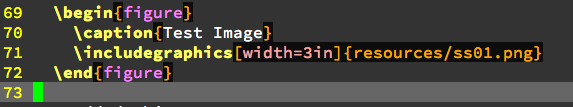
\includegraphics[width=3in]{resources/ss01.png}
  \caption{Test Image}
\end{figure}

I added this.

\newpage

\section{Section Four}
This is a new page of text.

\newpage

\begin{figure}
  \caption{Example DOT digraph}
  \label{dotgraph}
\end{figure}


Stuff
%% End Document Content
\end{document}
